\chapter{Future Work}

\section{Data collection}

\begin{itemize}
	\item Already performed: obtain REB approval for retrospective data collection
	\item Already performed: design data collection procedure, including data collection form, anonymization and parsing program
	\item Late January: meeting with Toronto Western Hospital research and clinical staff to initialize data collection process
	\item Early February: finalize data collection procedure and start mass data collection
	\item Late February: preliminary database establish at similar size scale of the Rotterdam dataset
	\item March to future: continued data collection
\end{itemize}

\section{Literature Algorithm Implementation}

\begin{itemize}
	\item February to March: Implement algorithms in literature for comparison against our approach
\end{itemize}

\section{Deep Learning Algorithm Design}

\begin{itemize}
	\item Current: A preliminary deep neural network design is in place, consisting of \iac{CNN} for spatial feature detection and \iac{LSTM} \ac{RNN} for temporal sequence feature detection. The features are concatenated and passed to a fully connected network for final output. 
	
	\begin{figure}[h]
		\centering
		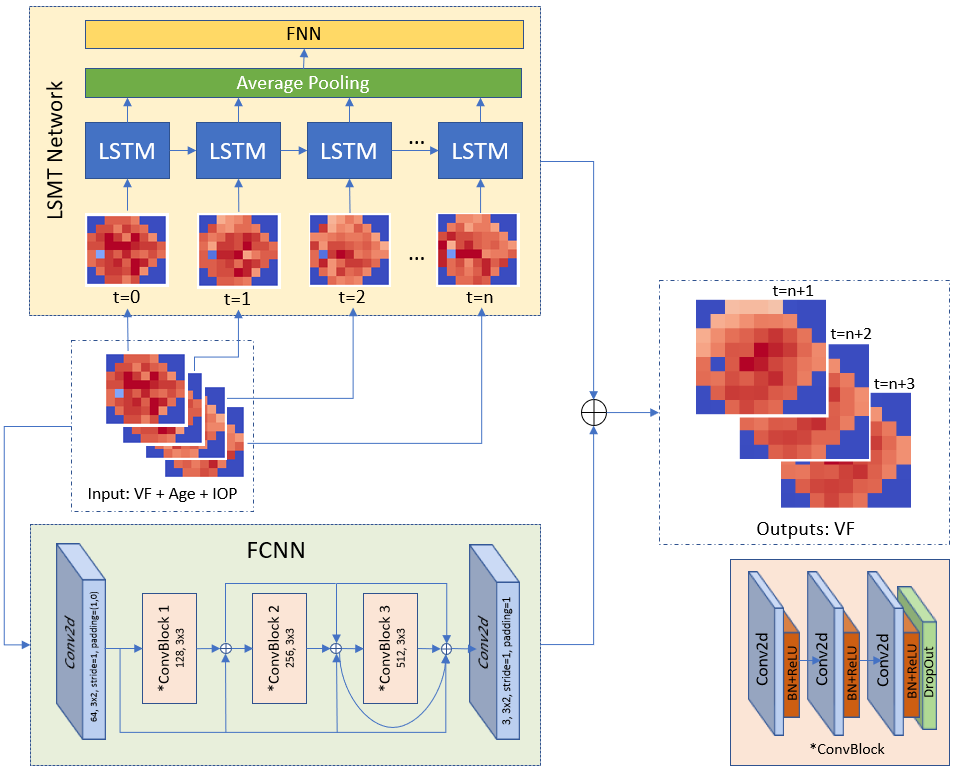
\includegraphics[width=\textwidth]{nn_struct}	\caption{Proposed neural network structure}
		\label{fig:nn_struct}
	\end{figure}

	\item February: Fix current issues present in the algorithm implementation and evaluate network performance against other methods.
	
	\item March: Preliminary testing of designed network on the collected Toronto dataset.
	
\end{itemize}

